%% LaTeX2e class for seminar theses
%% sections/deep learning methods.tex
%% 
%% Karlsruhe Institute of Technology
%% 
%%
%% Dr.-Ing. Fabian
%%
%% Version 1.0.2, 2020-05-07
%% A Survey on Deep Learning Architectures for Image-based Depth Reconstruction
\section{Introduction}
\label{ch:intro deep learning}

%% -------------------
%% | Example content |
%% -------------------
Estimating depth from RGB images is a long-standing ill-posed problem, which has been explored for decades. We will focus on the works which use deep learning techniques to estimate depth from one or multiple images. The goal is to estimate one or multiple depth maps, which can be from the same viewpoint as the input or from a new arbitrary viewpoint. In We can distinguish two main categories of methods. Methods in the first class (Section 3) mimic the traditional stereo-matching techniques by explicitly learning how to match, or put in correspondence, pixels across the input images. Such correspondences can then be converted into an optical flow or a disparity map, which in turn can be converted into depth at each pixel in the input image.  Instead, they learn a function that directly predicts depth (or disparity) at each pixel in the input image(s). This part is strongly influced by \href{https://arxiv.org/abs/1906.06113}{A Survey on Deep Learning Architectures for Image-based Depth Reconstruction}.

\subsection{category 1: stereo matching}
\label{stereo matching networks}
Performance comparison of deep learning-based multiview stereo matching algorithms on the KITTI 2015 benchmark. Accuracy and completeness refer, respectively, to the mean accuracy and mean completeness (the lower the better).
\begin{enumerate}
    \item  \href{https://arxiv.org/abs/1804.02505}{MVSNet: Depth Inference for Unstructured Multi-view Stereo}. \\
    Best performance on Dataset DTU\\
    \item   \href{https://arxiv.org/abs/1804.00650}{DeepMVS: Learning Multi-view Stereopsis}\\
    Best performance on Dataset ETH3D\\
\end{enumerate}




\subsection{category 2: depth estimation as regresion}
\label{stereo matching networks}
They consider a learned, view-based representation for depth reconstruction from
either n predefined viewpoints {v 1 , . . . , v n }, or from any arbitrary viewpoint specified by the user. Their goal is to learn a predictor f (see Section 2), which predicts depth map from an input I

\begin{enumerate}
    \item \href{https://arxiv.org/abs/1806.02446}{Deep ordinal regression network for monocular depth estimation}. \\
    Best performance for multi-view depth estimation on KITTI, Nr. 1 in 2018, Dataset KITTI \\ 
    \item \href{https://arxiv.org/abs/1702.02706}{Semi-Supervised Deep Learning for Monocular Depth Map Prediction}\\
    Nr1. multi-view, no implementation, Dataset KITTI
    
    \item \href{https://openaccess.thecvf.com/content_ECCV_2018/papers/Jianbo_Jiao_Look_Deeper_into_ECCV_2018_paper.pdf}{Look deeper into depth: Monocular depth estimation with semantic booster and attention-driven loss} best single view depth prediction on NYUDv2
    
    \item \href{https://github.com/nianticlabs/monodepth2
}{Digging Into Self-Supervised Monocular Depth Estimation} Best performance with multiple metrics, Rank 5 e.g. RMSE, Accuracy, Abs Rel 2019

    \item \href{https://paperswithcode.com/paper/self-supervised-monocular-trained-depth}{Self-supervised Monocular Trained Depth Estimation using Self-attention and Discrete Disparity Volume}
    Rank 1 # 2020
\end{enumerate}
Above ranking comes from \href{Rankings}{https://paperswithcode.com/sota/monocular-depth-estimation-on-kitti-eigen-1}





% \begin{equation}
% \label{eqn:lf_model1}
%     \mathcal{L}(x_{w}, o_i, \lambda) \quad x_w=(x_x, x_y,x_z), \quad o_1 = (o_x, o_y, o_z), \quad \lambda = (l_r,l_g,l_b)
% \end{equation}

% \begin{figure}
% \centering
% 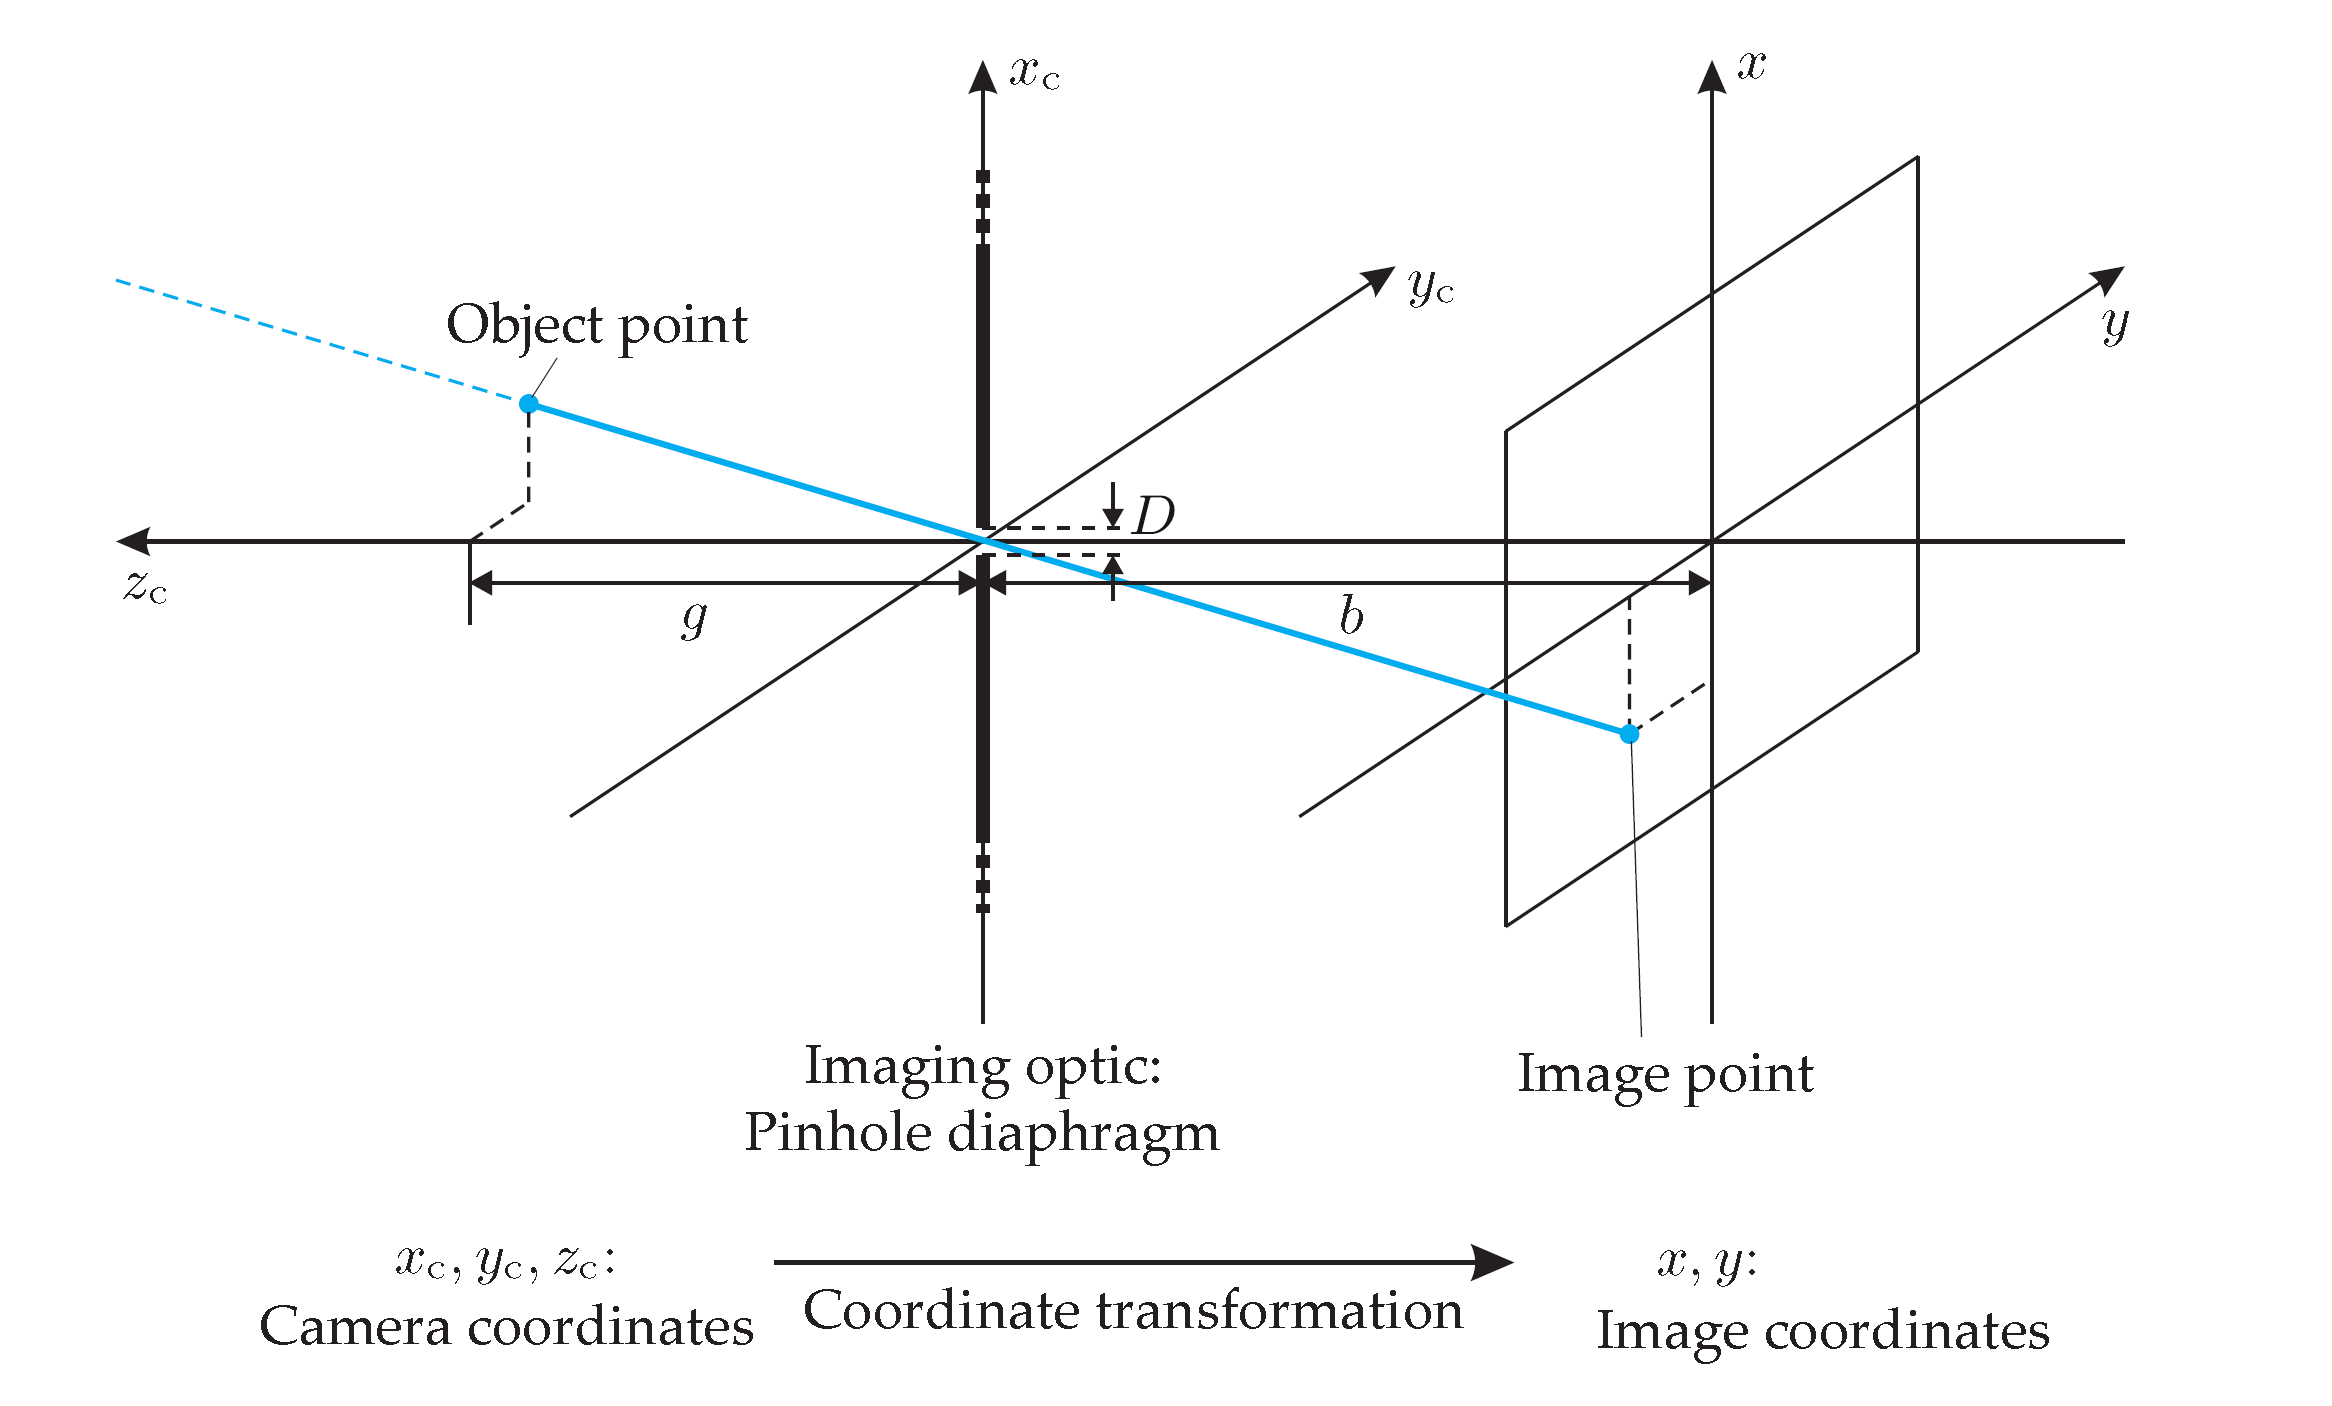
\includegraphics[width=15cm]{images/camera_model.PNG}
% \caption{pinhole camera model}
% \label{fig:pinhole camera model}
% \end{figure}
